\chapter{Review of Literature\label{ch:lit-review}}
There can be many techniques and approaches to address a problem. Many solutions can be developed to solve a single a problem. We studied a bunch of different approaches in the literature of SLR and analyzed them so that to study what benefit an approach over another. These approaches involved sub-unit based approach to extract hands from background, static gabor filter based approach to background subtraction, ESF descriptor approach to extract features and many more. A few of the major approaches that helped us to get a deeper insight and derive a strategy are given in below sections.

\section{Sub-unit based approach}
 This is a sub-unit based Sign language recognition culminating in a real time Kinect demonstration system. This approach uses different types of sub-units e.g. Location, Motion and Hand-shape sub-units tracked and identified by both 2D and 3D tracking data. These sub-units are then combined using a sign level classifier. Further two approaches are used for time-series processing. First is Markov Models (in form of DTW i.e. Dynamic Time Warping) to encode temporal changes in sub-units. Second is uses Sequential Pattern Boosting to apply discriminative feature selection at the same time as encoding temporal information. This approach is more robust and performs well in signer independent tests and improves accuracy from 54\% to 76\% and then to 85.1\% for signer independent tests. \cite{no1}


\begin{figure}[!htb]
	
	\minipage{0.9\textwidth}
	\caption{Sub-Unit Based Approach }\label{fig:image1}
	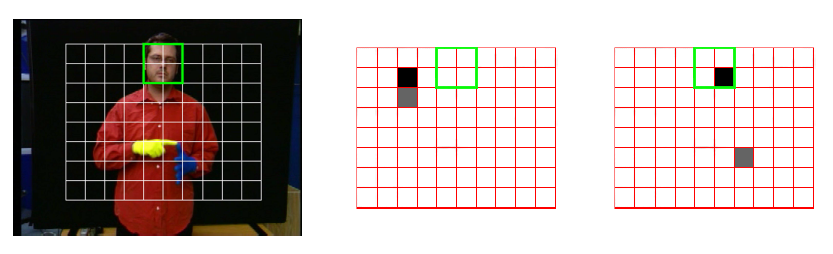
\includegraphics[height=3.4cm, width=15cm]{ThesisFigs/image1.png}
	
	\centering (a) Location based sub-units 
	
	\endminipage\hfill
	\minipage{0.4\textwidth}
	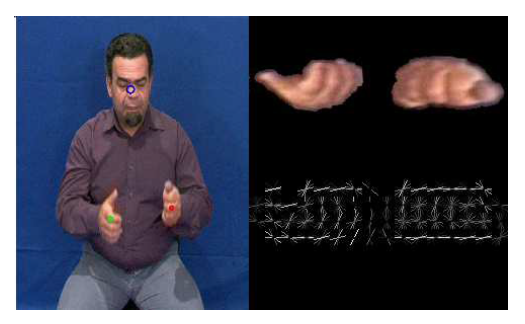
\includegraphics[height=3.2cm, width=\linewidth]{ThesisFigs/image2.png}
	(b) HOG Hand Shape descriptor
	\endminipage\hfill
	\minipage{0.4\textwidth}
	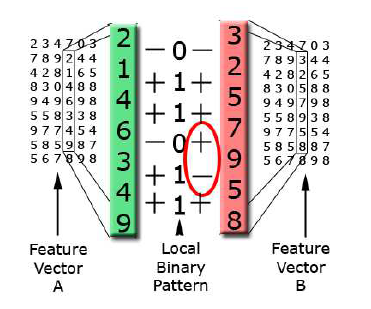
\includegraphics[height=3.2cm,width=\linewidth]{ThesisFigs/image3.png}
	(c) LBP Motion based descriptors 
	\endminipage\hfill
	
\end{figure}


\section{Static Gabor filter based approach}
 In this Research, Kinect Camera was used for input purposes keeping in mind that in this case input were images of static signs. Hand was segmented based on depth information right from the Kinect. Then hand shape features used are based on Gabor filtering of intensity and depth images. The purpose of using Gabor filter was that Gabor filter is apt at capturing contrast on image patch at different scales. Lately Random Forest was used for training and classification purposes on feature values obtained by Gabor filtering. A mean precision of 75\% was obtained following the considered approach.\cite{no2}

\section{ESF descriptors}
 Another approach used in previous computer scientists used ESF descriptors to unique identify different signs (static images). They used ToF (Time of Flight) cameras but techniques works perfectly fine with Kinect inputs just needs to be configured accordingly. ESF features were extracted from training samples and then trained with MLRF (Multi layered Random Forest). This is a simple approach which sacrifices accuracy for quick results. An accuracy of 85\% was observed practicing this approach.\cite{no3}

\section{Skin Intensity based hand-feature extraction}
 This approach proposes a technique that first takes intensity of skin color of sign and then segment the face, hand and elbow based on these intensity values. There are water-marks on the interface. In the few starting frames, signer has to place his elbow and hands on the specified water-marks. With these frames, algorithm is capable of finding the range of intensities of skin pixels. Then segment each of the frame to get the hand, elbow and face-region. The flatness of hand-region, CG of hand w.r.t face, area of hand, the direction of hand motion (depicted in below diagram) and the direction of hand-region by elbow angle.\cite{no4}


\begin{figure}[!htb]
	\begin{center}
		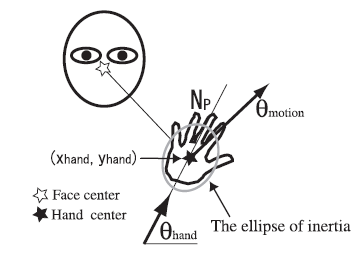
\includegraphics[height=4cm, width=8cm]{ThesisFigs/image0}
		\caption{Skin Intensity based hand-feature extraction}\label{fig:image0}
	\end{center}
	
\end{figure}

Feature set is fed to HMM (Hidden Markov Model).Which is used for prediction of signs.

\section{DTW based approach}
This approach is the most similar one to the project being presented; in this the whole words are being translated from sign videos not gestures. For this purpose, system takes the input from the Kinect as a series of frames. Then for all these frames, joints of interest are extracted which are the joints of two fingers in the ideal case. The distance between these joints and the Cartesian coordinates of the joints of interest (taking the origin at the center of the spine of signer’s body) are taken as features. As these features are extracted now a time series is built for the whole video. Later the time series is trained using the DTW. DTW matches the frames in the two (trained time-series and test time-series) and then predicts to the class with which it has lowest error. DTW on the backend uses an HMM. The most prominent feature of this pilot study was that the signs are taken from Pakistan Sign Language. \cite{no5}

\begin{figure}[!htb]
	\begin{center}
		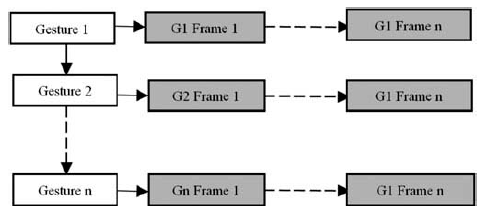
\includegraphics[height=5cm, width=12cm]{ThesisFigs/differentgesture}
		\caption{Different Gesture Format}\label{fig:Different Gesture}
	\end{center}
\end{figure}
The following picture demonstrates the dataset shape and organization





